%# -*- coding: utf-8-unix -*-
%%==================================================
%% chapter02.tex for SJTU Master Thesis
%% based on CASthesis
%% modified by wei.jianwen@gmail.com
%% Encoding: UTF-8
%%==================================================

\chapter{ 在线自组织哈希}
\label{chap:SOH}

在哈希领域中,大部分哈希方法如局部敏感哈希(Locality-Sensitive Hashing,LSH)等,使用超平面作为哈希函数。在这些方法中,首先,一些按照特点方式生成的超平面将数据空间切分成几个不重叠的区域;之后,处在每个区域内数据点被量化成一个二值编码。

同时,一些不依靠超平面的哈希方法也被提了出来。如球哈希(Spherical Hashing)和K均值哈希(Kmeans Hashing, KMH)。相比于使用超平面的哈希方法,这些方法的优点在于能定义更加紧密的不重叠区域,从而提升哈希的效果。KMH提出了一个几何视角来比较哈希和量化(Quantization)这两种方法,即任何使用正交的超平面来切割空间的哈希方法,都可以看成是使用一个超正方体的顶点作为量化中心的量化方法。KMH使用EM算法来优化量化误差(quantization error)和亲和误差(affinity error)两种误差的和。凭借K均值量化的适应性和亲和保持能力,KMH的效果超过了绝大部分基于超平面的哈希方法。

虽然这些哈希方法取得了优良的效果,但是他们在两个特点环境下仍存在问题。首先,存储在分布式系统上的海量大数据根本无法存入计算机内存中;其次,很多应用的数据以流式产生,而这些方法必须将所有数据积累起来再学习哈希函数。

为了解决这些问题,两个在线哈希技术被提出,分别是在线哈希(OKH)和在线梗概哈希(OSH)。这两种方法凭借在线学习的方式,解决了上述两个问题。但是,他们是基于超平面的哈希方法,存在着分割空间能力弱的问题。所以,本文在本章节提出一种基于在线自组织映射网络的哈希方法——在线自组织哈希(Online Self-Organizing Hashing, SOH)。该哈希方法有两点好处:
 \begin{itemize}
 	\item 该方法假设数据以流式的方法到来,并在收取到任意数据后即可立即更新模型。该方法特别适合数据量或数据维度极大的大数据应用。
 	\item 在构造超正方体的过程中,超正方体顶点的拓扑结构可以被很好的保持。因此,该方法不仅有比基于超平面哈希的优势,还比KMH具有更低的量化误差和亲和误差。
 \end{itemize}

本章首先会介绍与在线自组织哈希相关的工作如K均值哈希、自组织映射网络的相关知识,再详细介绍该方法的算法细节。最后是实验结果和结论部分。

\section{相关工作}
在该部分,本文会简要介绍K均值哈希(Kmeans Hashing,KMH)、自组织映射网络(Self Organizing-Map,SOM)两种技术。

\subsection{K均值哈希}
K均值哈希是一个基于K均值聚类方法的能保持数据与量化中心亲和的哈希方法。该方法结合了哈希与量化技术,非常新颖。
给定一个数据集 $\mathbf{X} = [\mathbf{x}_{1}, \mathbf{x}_{2},...,\mathbf{x}_{n}]^{T} \in R^{n\times d}$ ,
KMH首先构建一系列向量 $\mathbf{W} = [\mathbf{w}_{1},  \mathbf{w}_{2}, ..., \mathbf{w}_{k}]^{T} \in R^{k\times d}$.
该向量集合$\mathbf{W}$ 被叫做码表,其中 $\mathbf{w}_{i}$是一个编码值。每个编码值同时又一个二值码$\mathbf{y}_{i}\in \{0, 1\}^{b}$,其中 $b$ 代表了二值编码的长度,所以可得出$k=2^{b}$。之后KMH将任意数据点$\mathbf{x}$映射到一个编码值$\mathbf{w}_{i(\mathbf{x})}$同时最小化下面的目标函数:
\begin{equation}\label{eq:4}
E = E_{\mathrm{quan}} + \rho E_{\mathrm{aff}}.
\end{equation}
其中$E_{\mathrm{quan}}$是经典的K均值算法的平均\emph{量化误差}:
\begin{equation}\label{eq:1}
E_{\mathrm{quan}} = \frac{1}{n}\sum_{\mathbf{x}\in \mathbf{X}} ||\mathbf{x}-\mathbf{w}_{i(\mathbf{x})}||^{2},
\end{equation}
其中$E_{\mathrm{aff}}$是由于使用二值编码来近似聚类中心所导致的\emph{亲和误差}:
\begin{equation}
E_{\mathrm{aff}}= \sum_{i=1}^{k}\sum_{j=1}^{k}w_{ij}(d(\mathbf{w}_{i}, \mathbf{w}_{j}) - d_{h}(i, j))^2.
\end{equation}
在这里,$w_{ij} = n_{i}n_{j}/n^{2}$. $n_{i}$和$n_{j}$是索引值为$i$和$j$的样本数量。 $d_{h}$是两个二值编码$\mathbf{y}_{i}$和$\mathbf{y}_{j}$的基于海明值的距离:
\begin{equation}\label{eq:d_h}
d_{h}(i,j) \triangleq s \cdot h^{\frac{1}{2}}(\mathbf{y}_{i},\mathbf{y}_{j}),
\end{equation}
其中$s$使用过主成分哈希(PCAH)所确定的一个缩放常量。 $h$代表海明距离。
KMH使用类似于K均值算法中使用的EM算法来优化这个目标函数。

\subsection{自组织映射网络}
\begin{algorithm}[tb]
	\caption{自组织映射算法}
	\label{alg:som}
	\begin{algorithmic}
		\Repeat
		\State 1.在每个时间点$t$, 输入一个$\mathbf{x}(t)$, 并选择距离$\mathbf{x}(t)$最近的神经元。
		\begin{equation}\label{eq:5}
		v(t) = \mathrm{arg\ min}_{1 \leq i \leq k} || \mathbf{x}(t) - \mathbf{w}_{i}(t)||
		\end{equation}
		\State 2.更新所有神经元的权值。
		\begin{equation}\label{eq:6}
		\Delta\mathbf{w}_{i}(t) = \alpha(t)\eta(v, i, t)\big(\mathbf{x}(t) - \mathbf{w}_{i}(t)\big)
		\end{equation}
		\Until{网络收敛}
	\end{algorithmic}
\end{algorithm}
自组织映射网络(SOM)是一个能对高位数据进行拓扑结构保持的有效量化的无监督神经网络。SOM使用一系列的组织在二维平面上的神经元,来组成一个多边形,用来近似$d$维的原始输入数据$\mathbf{X}$的拓扑结构。这里本文假设神经元的维度为$b$ ,共有$k$个神经元。由此在该空间中得到一个向量的集合$\mathbf{R} = [\mathbf{r}_{1},  \mathbf{r}_{2}, ..., \mathbf{r}_{k}]^{T} \in R^{k\times b}$。在学习的初始阶段,所有的权值$\mathbf{W} = [\mathbf{w}_{1},  \mathbf{w}_{2}, ..., \mathbf{w}_{k}]^{T} \in R^{k\times d}$被初始化为随机的数值。其中,$\mathbf{w}_{i}$是神经元$i$的权值向量。该向量和输入数据$\mathbf{x}$的维度$d$一致。然后,自组织映射算法重复算法\ref{alg:som}中的步骤。$\eta(v, i, t)$是邻接函数。一般来说,我们可以使用任意形式的邻接函数,但是在实际问题中,高斯函数是最常用的:
\begin{equation}\label{eq:7}
\eta(v, i, t) = exp\Big(-\frac{Dist(\mathbf{r}_{v} , \mathbf{r}_{i})}{2\sigma(t)^{2}}\Big),
\end{equation}
\begin{equation}\label{eq:8}
\sigma(t) = \sigma_{0}exp(-\frac{t}{\lambda}),
\end{equation}
公式\ref{eq:6}中的学习率$\alpha(t)$同样是一个指数形式的衰减函数,用来确保SOM算法最终收敛:
\begin{equation}\label{eq:9}
\alpha(t) = \alpha_{0}exp(-\frac{t}{\lambda}),
\end{equation}
当SOM的节点数较少时,该算法与K均值算法类似。但SOM的网络很大时,网络的拓扑结构就会呈现出与数据的拓扑结构近似的性质。因此,基于SOM的哈希方法相比于使用一般方法来优化公式\ref{eq:4}的算法,理应具有更优的亲和误差。

\section{算法介绍}
\subsection{在线自组织哈希}
在线自组织哈希(SOH)的研究动机来自SOM算法。SOH以在线自组织的形式来量化特征空间,而不是使用离线的EM算法的形式。并且,SOH并不是采用传统的二维或一维的网络映射,而是将神经元节点构建成一个$b$维的超立方体。 该超立方体具有$k=2^{b}$个顶点,从而每个顶点都有一个唯一的$b$比特位的二值编码$\mathbf{y}_{i}$。该方法在每一步最小化下面的亲和保持采样函数:
\begin{equation}\label{objective_soh}
\begin{split}
E(t) = \sum_{i=1}^{k} \eta(v, i, t) \big( ||\mathbf{x}(t) - \mathbf{w}_{i}||^{2} + \beta  E_{\mathrm{aff}}(\mathbf{w}_{i})\big)
\end{split}
\end{equation}
其中$\beta$是一个固定的权值。
\begin{equation}\label{E_aff_w}
E_{\mathrm{aff}}(\mathbf{w}_{i}) =  \sum_{j=1}^{k}(d(\mathbf{w}_{i}, \mathbf{w}_{j}) - d_{h}(i, j))^{2}
\end{equation}
由此可以推导出算法\ref{alg:som}的第二步中新的更新公式:
\begin{equation}\label{eq_newupdate}
\Delta\mathbf{w}_{i}(t) =   \alpha(t)\eta(v, i, t)\big(\mathbf{x}(t) - \mathbf{w}_{i}(t) -  \beta \frac{\partial E_{\mathrm{aff}}(\mathbf{w}_{i})}{\partial \mathbf{w}_{i}}\big)
\end{equation}
由公式\ref{E_aff_w}可以推导出:
\begin{equation}\label{eq_partial}
\frac{\partial E_{\mathrm{aff}}}{\partial \mathbf{w}_{i}} = \sum_{j=1}^{k}4 \Big(1 - \frac{d_{h}(i, j)}{d(\mathbf{w}_{i}, \mathbf{w}_{j})} \Big)(\mathbf{w}_{i} - \mathbf{w}_{j})
\end{equation}

在每一次迭代过程中,该方法需要调整超立方体的顶点。调整方法按照公式\ref{eq_newupdate}和公式\ref{eq_partial}所述。在公式\ref{eq:7}中,需要计算超立方体上两个顶点的距离,该距离使用顶点的二值编码的海明距离的平方来表示:
\begin{equation}\label{10}
Dist(\mathbf{r}_{v} , \mathbf{r}_{i}) = h(\mathbf{y}_{v}, \mathbf{y}_{i})^2,
\end{equation}

通过整个学习过程,超立方体的顶点的权值最终收敛。数据集中的每个样本被赋予一个二值编码,该二值编码为距离该样本最近的超立方体顶点的二值编码。

\subsection{模型初始化以及参数$s$的选取}
KMH通过主成分哈希的方法来初始化每个超立方体顶点的二值编码。于KMH不同,由于本文所提出的SOH可以自适应的近似数据的分布,所以通过任意方法初始化仍可以达到相同的效果。在实际使用时,SOH的超立方体以一个标准超正方体的方式来初始化,即超立方体的每条边都与坐标轴平行,如图 \ref{init}所示。
\begin{figure}[ht]
	\begin{center}
		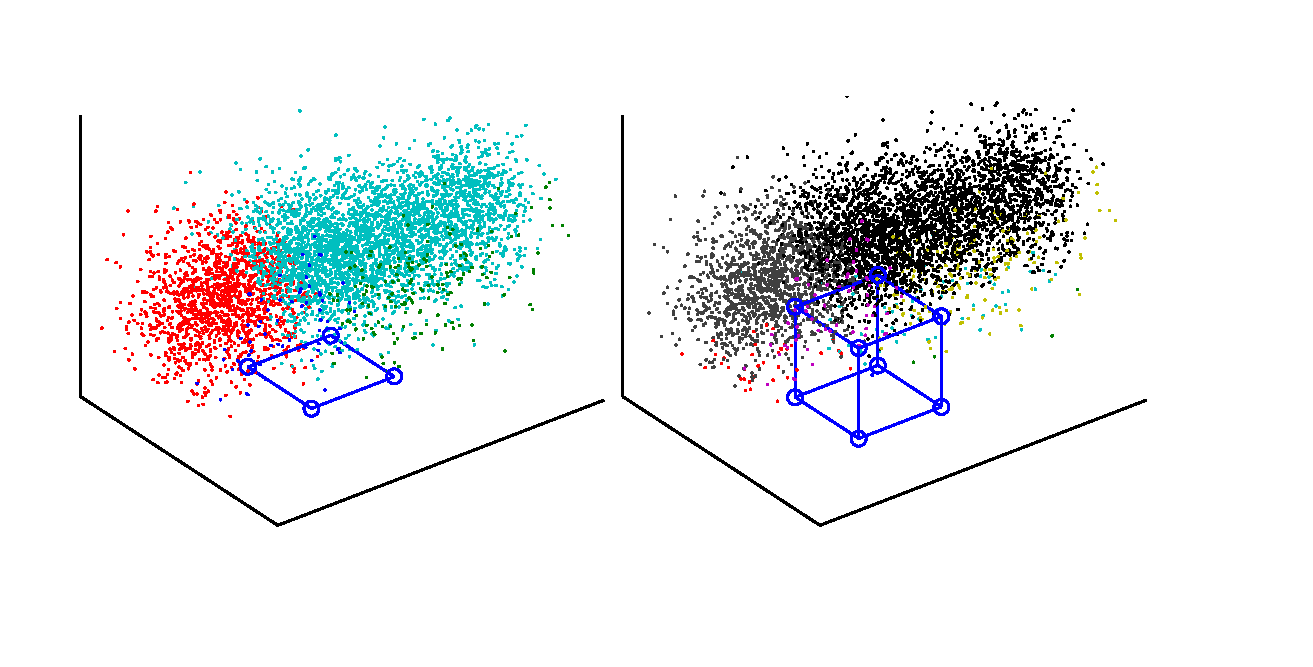
\includegraphics[width=0.76\columnwidth]{init}
		\caption{当数据特征空间为三维,超立方体为二维和三维时,SOH初始化方法的几何展示。图中数据样本通过随机采样产生,且均值并不在坐标原点上。}
		\label{init}
	\end{center}
\end{figure}

公式\ref{eq:d_h}中$d_{h}(i, j)$里面的缩放参数$s$最初通过随机的方式初始化。因为公式\ref{E_aff_w}是一个关于$s$的二次函数,所以可以解出一个闭式解$\hat{s}$出来。在每次迭代更新超立方体顶点前,参数$s$可以直接按照下述方法直接更新:
\begin{equation}\label{optimal_s}
\hat{s} = \frac{\sum_{i}\sum_{j}d(\mathbf{w}_{i}, \mathbf{w}_{j})h^{\frac{1}{2}}(i,j)}{\sum_{i}\sum_{j}h(i,j)}
\end{equation}
由此,在线自组织哈希的全部流程可以通过算法\ref{alg:soh}所述方式完成:
\begin{algorithm}[tb]
	\caption{在线自组织哈希}
	\label{alg:soh}
	\begin{algorithmic}
		\State 初始化超立方体的顶点以及参数$s$。
		\For{t = 1,2,...}
		\State 1.按照公式\ref{optimal_s}来更新$s$。
		\State 2.输入一个样本$\mathbf{x}(t)$,根据公式\ref{eq:5}选择距离样本最近的超立方体顶点。
		\State 3.根据公式\ref{eq_newupdate}和公式\ref{eq_partial}更新超立方体的全部顶点。
		\EndFor
	\end{algorithmic}
\end{algorithm}

\subsection{一般化到乘积空间}

\begin{figure}[ht]
	\begin{center}
		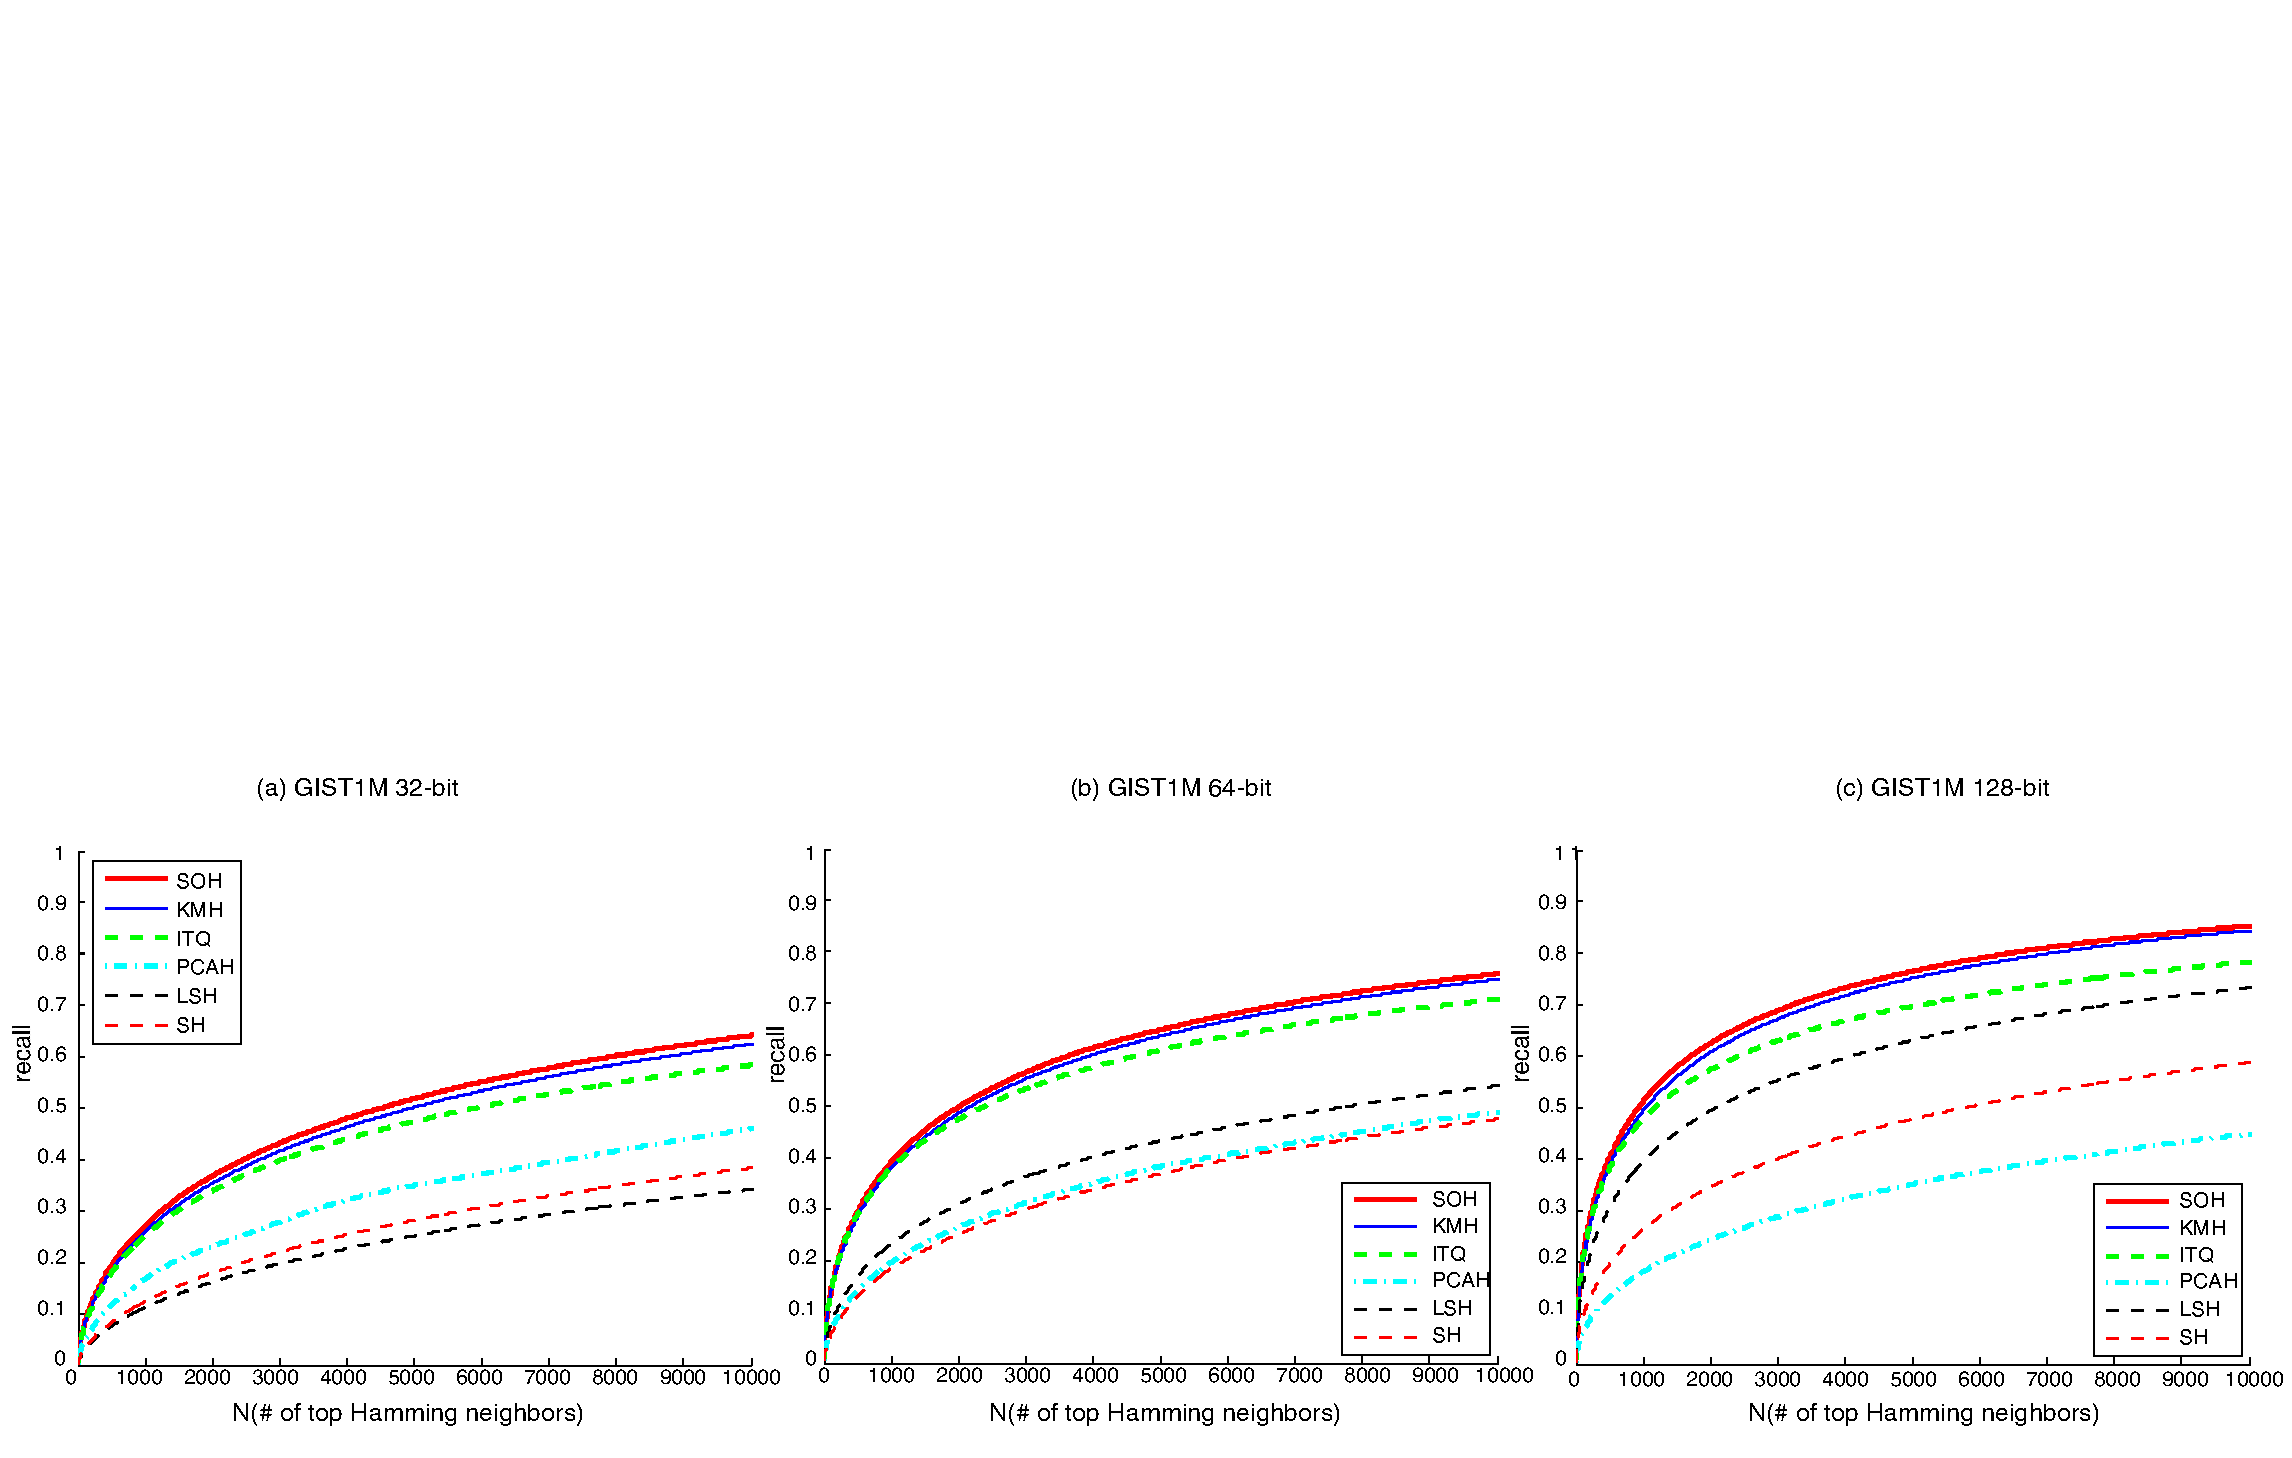
\includegraphics[width=1\columnwidth]{batch_compare}
		\caption{(a)(b)(c)GIST1M数据集上使用32,64,128比特位的召回曲线。本文的SOH和KMH在32和64比特位下均设定b=4,在128比特位下设定b=8。在该幅图中,正样本是欧式距离最小的前K=10的近邻点。该幅图使用彩色版本观看最佳。  }
		\label{batch_compare}
	\end{center}
\end{figure}
与KMH相似,当比特位$b$很大时,本文中的SOH也可以一般化到乘积空间中去。例如,随机旋转的方法可以将原始空间分解成多个乘积空间,由此可以像局部敏感哈希一样得到多个查找表。然而,使用随机旋转再分解的方法会导致单个查找表的效果难以保证。如果想得到最好的分解方式,可以按照文献\cite{ge2014optimized}所介绍的特征值分配的方法来分解。特征值分配方法需要在数据集上进行主成分分析,为了减少主成分分析所带来的巨大计算量,文献\cite{leng2015online} 中的数据梗概法可以以在线学习的方式进行主成分分析。在实际操作中,在全部数据集上进行在线主成分分析是没必要的。所以,可以只对一小部分数据进行主成分分析,接着得到一个比较好的空间分解,最后再进行SOH的学习。

\section{实验结果}
在本节中,为了展现SOH的良好性能,我们首先比较与直接应用SGD以优化公式\ref{4}(我们称该方法为KMH-SGD)。 之后,一些列当前最好的哈希方法也作为比较对象参与比较。 对比实验分为批量设置和在线设置两种,分别用于验证有效性和效率。 我们将原始的数据空间分解为$M$个子空间,每个子码表有$b$个比特位。这$M$个二值编码被连接成一个$ M\cdot b$比特位的二值编码。 通过控制参数$\lambda $,该算法可以确保在每个样本都被呈现一次后收敛。
对于试验中使用的超参数,在$b=2$时$\beta = 0.5$,  在$b=4$时$\beta = 0.1$, 在$b=8$时$\beta = 0.01$。其他的超参数统一设定为$\sigma_{0} = 1$, $\alpha_{0} = 0.05$。
\begin{figure}[t]
	\begin{center}
		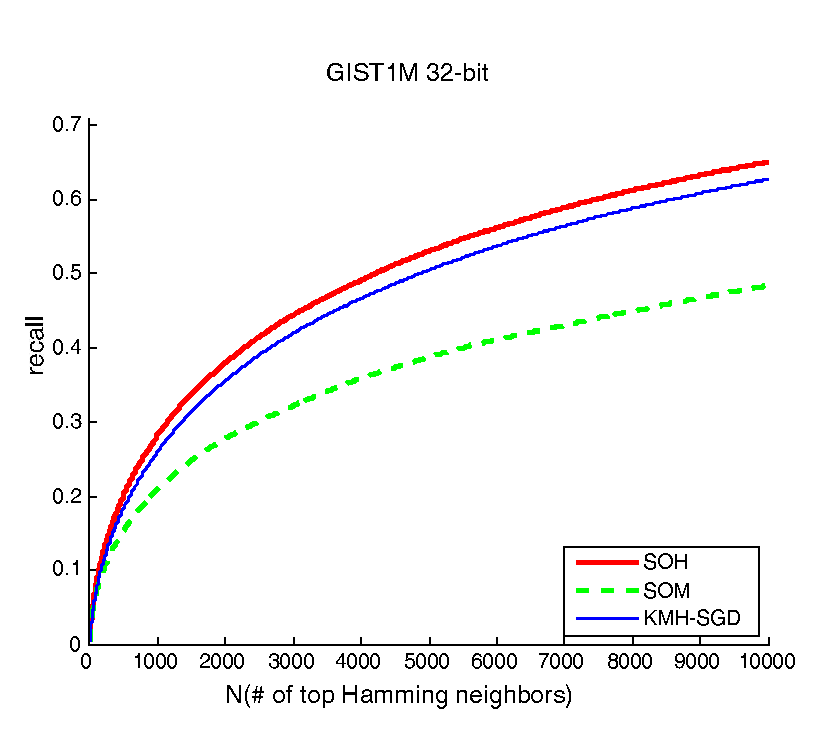
\includegraphics[width=0.76\columnwidth]{online_compare}
		\caption{GIST1M在三种在线算法上的召回曲线。在该幅图中,正样本是欧式距离最小的前K=10的近邻点。本文的SOH方法设定b = 4。 }
		\label{somkmeans}
	\end{center}
\end{figure}
\subsection{数据集和评价标准}
检索效果通过两个公开数据集来评测,它们分别是:SIFT1M\footnote{http://corpus-texmex.irisa.fr}和GIST1M\footnote{http://groups.csail.mit.edu/vision/TinyImages/}。
SIFT1M包含100万个128维的SIFT特征向量\cite{lowe2004distinctive}以及10000个检索向量。 GIST1M包含100万个384维的GIST特征向量\cite{oliva2001modeling}以及10000个独立采样出的检索向量。
对于这两个数据集,在批量设置实验中,我们随机采样10万个数据样本进行训练,而在在线设置中,全部100万的训练样本都被用来进行训练。
评测时,每一个检索向量都召回全部数据中的前$K$个欧氏距离的最近邻。在大多数实验里,$K$被设定为10。同时,本文还做了一个专门针对$K$的实验,在该实验中,不同$K$下的检索结果被一一评估,用以说明$K$的选取并不会影响实验的一致性。
在批量设置下,本文采用海明排序来生成召回率结果。在在线设置下,检索效果使用平均精准度(mean average precision,MAP)来衡量。本实验的实验环境为因特尔i5-4430@3.0GHz处理器,以及16GB内存。
\subsection{Results and Discussions}
首先,我们将本文提出的SOH算法与KMH-SGD比较。除此之外,不使用亲和保持 (算法 \ref{alg:som})的普通SOM算法也作为对比方法,以用于证明亲和保持的重要性。
\begin{figure}[t]
	\begin{center}
		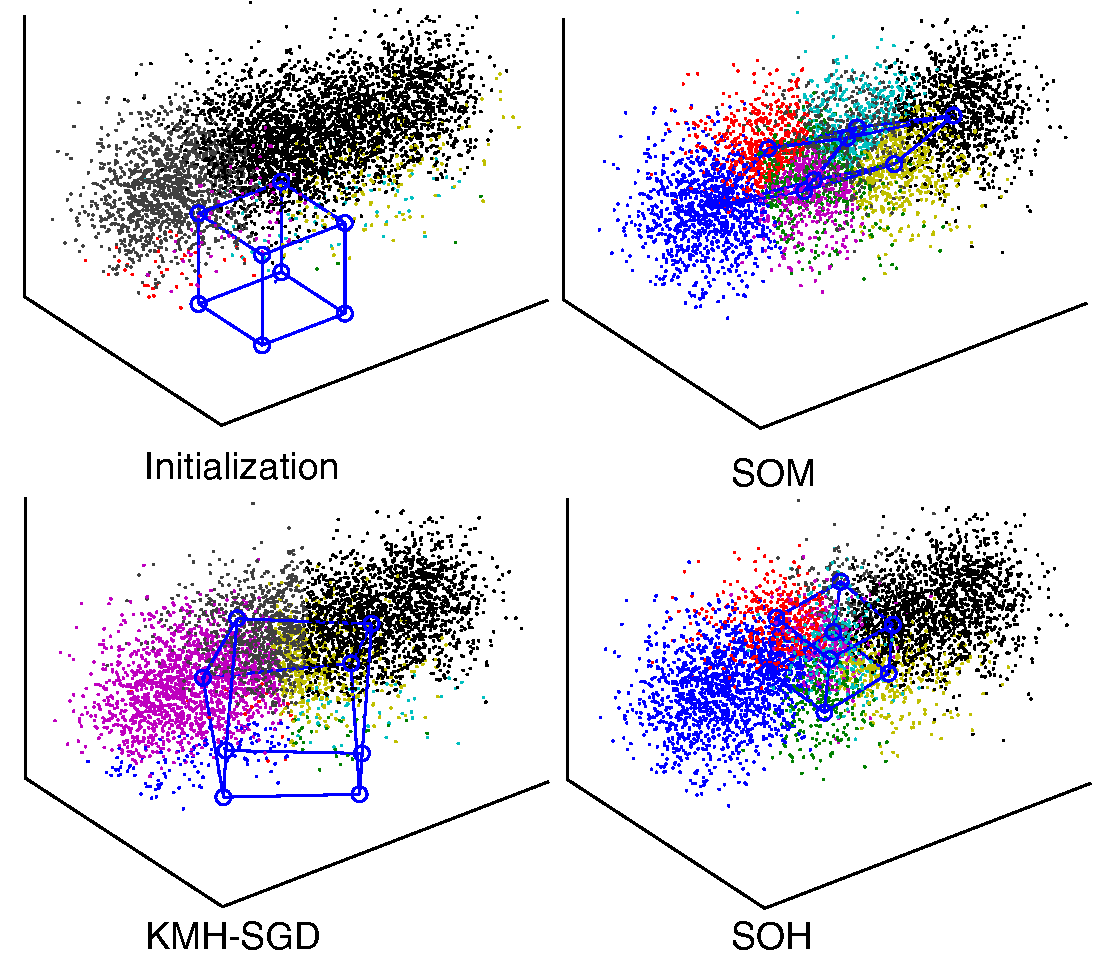
\includegraphics[width=0.76\columnwidth]{SOHvsOnlineKMS}
		\caption{SOM,KMH-SGD,SOH三种方法在数据维度与超立方体维度均为3维时的几何展示。图中显示的数据均为随机采样获得,且数据的中心店不在坐标系原点。该幅图使用彩色版本观看最佳。}
		\label{somall_2}
	\end{center}
\end{figure}
图\ref{somkmeans}展示了SIFT1M数据集在64比特位下的对比结果(M = 16个子空间)。可以很容易的发现,普通的SOM算法表现的非常差。KMH-SGD算法比SOM算法稍好,但是仍然差于SOH。为了理解为什么这两种方法比SOH效果要差,我们随机采样了5000个数据点,数据点的均值不为0。之后,我们在该数据集上使用上述三种算法分别训练三个不同的模型,模型的比特位$b=3$。我们将最终的超立方体可视化展示在图\ref{somall_2}中。
可以发现,SOM的立方体很好的近似了数据的真实分布。但是当数据不服从均匀分布时,这个立方体塌陷了。在这种塌陷情况下,两个海明距离很小的顶点,此时在数据空间中的欧式距离很大,从而导致了较大的亲和误差。

与SOM不同,KMH-SGD由于存在亲和保持特性,它的立方体的亲和误差很小。但是,由于该方法采用一般的随机梯度下降算法,导致很容易过早的陷入局部最优。尤其是在初始化较差的情况下,很多立方体顶点没有最近邻的数据点,从而导致在迭代优化时,这些顶点永远也不会被更新。当数据的均值非0时,该问题会变得更加严重。如图\ref{somall_2}所示,该方法的立方体虽然保持了较好的形态,但是很显然它没有很好的近似数据的真实分布,从而导致较大的量化误差。

本文提出的SOH通过考虑上面两种问题,首先包含了亲和保持,其次使用SOM算法,从而使得该算法既能很好的近似数据的真实分布,又能有很小的亲和误差。从而在最终的检索效果上达到最优。

接下来,在批量设置下,我们与当前最好的一些列哈希方法做对比试验,如LSH \cite{gionis1999similarity}, Spectral Hashing (SH) \cite{weiss2009spectral}, KMH \cite{he2013k}, PCAH and ITQ \cite{gong2013iterative}。哈希比特位从32到128,$K$从1到100都是本实验的可变参数,从而可以得到一系列全面的对比结果。当$K=10$时,图\ref{batch_compare}展示了全部算法的召回曲线。很明显,本文的SOH算法在任何一个比特位上的检索效果都超过了其他算法,从而可以得出SOH算法是一个稳定的有效算法的结论。在图\ref{fig_k}中,$K$的取值从1到100变化,在不同的$K$下,本文的SOH算法与KMH和ITQ进行比较。可以再一次看到,本文的SOH算法一直要优于其他两种算法。
\begin{figure}[ht]
	\begin{center}
		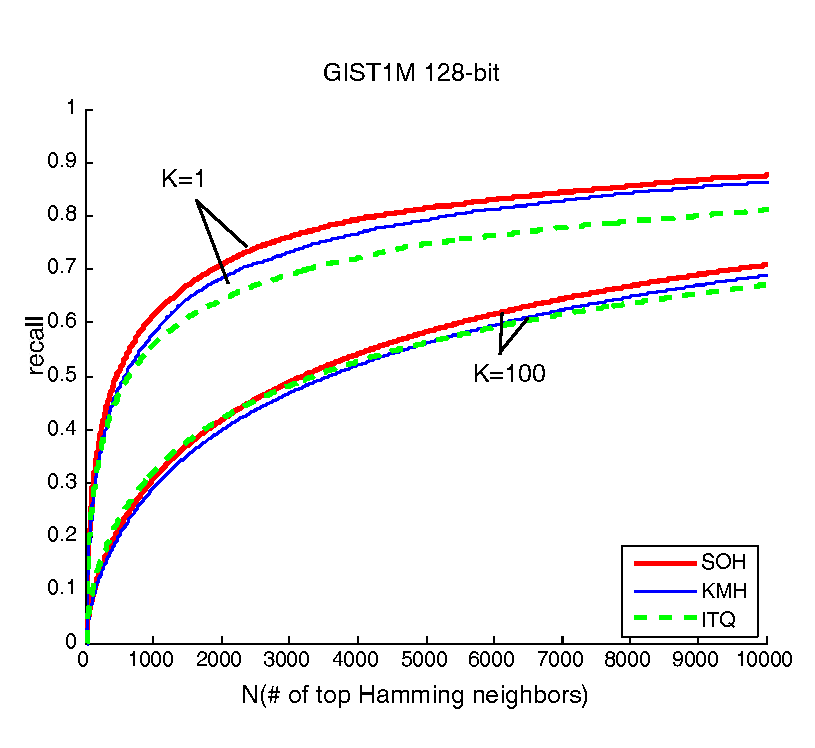
\includegraphics[width=0.76\columnwidth]{K}
		\caption{GIST1M数据集在128比特位以及不同的K(1, 100)下的对比结果。}
		\label{fig_k}
	\end{center}
\end{figure}
\begin{figure*}[ht]
	\begin{center}
		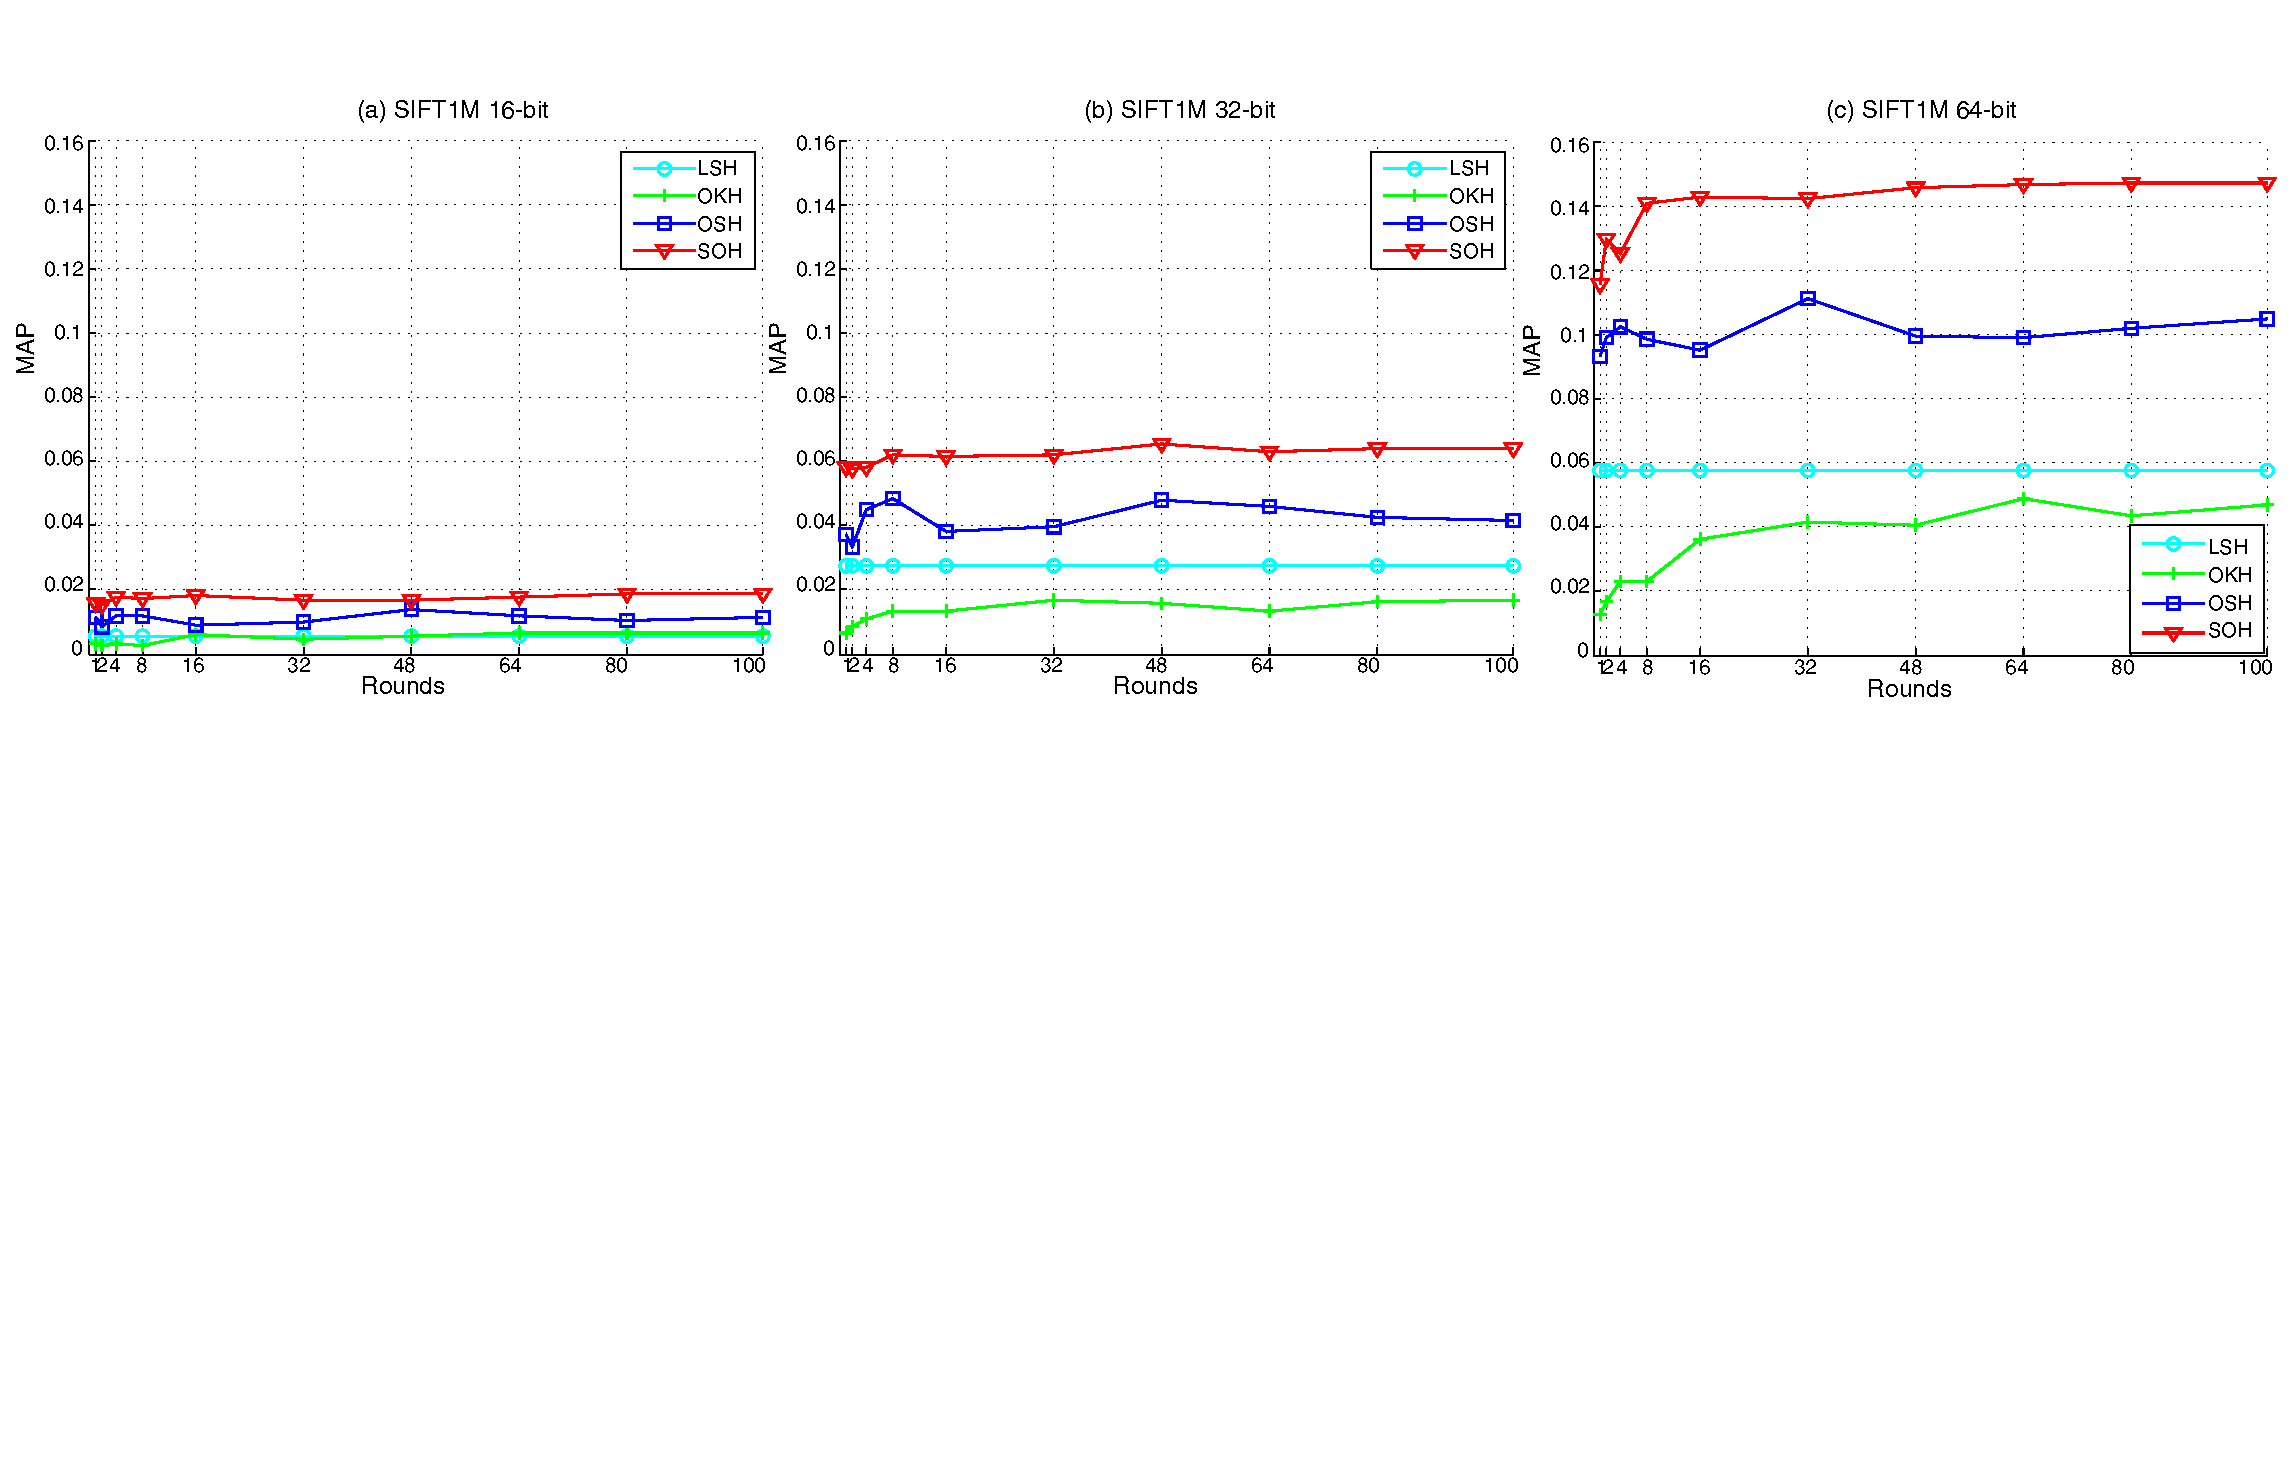
\includegraphics[width=0.92\textwidth]{onlinerst}
		\caption{(a)(b)(c)SIFT1M数据集上使用16,32,64比特位的MAP曲线。本文的SOH在16和32比特位下均设定b=2,在64比特位下设定b=4。在该幅图中,正样本是欧式距离最小的前K=10的近邻点。该幅图使用彩色版本观看最佳。 }
		\label{compare_online}
	\end{center}
\end{figure*}

一些列当前最好的在线哈希算法也是本文的对比对象。本文选择了OKH \cite{huang2013online}, OSH \cite{leng2015online}和LSH三种算法作为对比算法。实验同样在SIFT1M和GIST1M两个数据集上进行。为了体现在线学习的特点,训练数据被平均分成了100份。在训练时,模型以一份数据为单位进行迭代训练。MAP值在特点的迭代次数后计算。由此,本文的SOH和三种对比算法可以分别得到四个关于迭代次数的MAP曲线,通过比较这些MAP曲线,即可得出不同算法的相对效果的实验结果。对于本文的SOH,我们仅使用1份训练数据(10000个样本)来进行主成分分析投影的学习,学习方式为基于数据梗概的在线学习方法。在得到了主成分分析结果后,我们按照特征值分配的方法将数据空间分解。图 \ref{compare_online}展示了这4种方法在SIFT1M数据集上的比较结果。结果分为16,32,64比特位。可以看到,本文提出的SOH在任意比特位上,都大幅度超过了三种对比算法。而且我们可以发现,OSH算法的稳定性并不好,这是因为该算法使用随机的主成分投影。与之不同的是,本文提出的SOH算法在大部分实验里,检索效果都能随着迭代次数的增加而稳步提升。

最后,本文展示了关于训练时间的对比结果。在SIFT1M数据集上,我们先去1份数据(10000个样本点)进行训练,来比较不同算法在这一份数据上所要花费的时间。虽然在检索准确率上,KMH的效果接近本文提出的算法,但是由于多次在全量数据上的迭代,该算法需要更多的时间。对于不同比特位长度和子空间长度的对比结果展示在表格\ref{traintime-table}中。很明显,本文提出的SOH在计算法速度上是KMH的5倍左右。
\begin{table}[ht]
	\caption{SOH和KMH两种方法在SIFT1M数据集上关于不同比特位长度的训练时间的比较(10000个样本点)。}
	\label{traintime-table}
	\begin{center}
		\begin{small}
			\begin{sc}
				\begin{tabular}{lcccr}
					\hline
					比特位 & 子空间比特位 & KMH(s)& SOH(s) \\
					\hline
					32    & 2 & 20.04& 5.94\\
					32    & 4 & 76.10& 7.07\\
					64    & 4 & 74.46& 14.42\\
					64    & 8 & 944.16& 152.71\\
					128   & 8 & 989.27& 241.21\\
					\hline
				\end{tabular}
			\end{sc}
		\end{small}
	\end{center}
\end{table}